\documentclass[]{book}
\usepackage{lmodern}
\usepackage{amssymb,amsmath}
\usepackage{ifxetex,ifluatex}
\usepackage{fixltx2e} % provides \textsubscript
\ifnum 0\ifxetex 1\fi\ifluatex 1\fi=0 % if pdftex
  \usepackage[T1]{fontenc}
  \usepackage[utf8]{inputenc}
\else % if luatex or xelatex
  \ifxetex
    \usepackage{mathspec}
  \else
    \usepackage{fontspec}
  \fi
  \defaultfontfeatures{Ligatures=TeX,Scale=MatchLowercase}
\fi
% use upquote if available, for straight quotes in verbatim environments
\IfFileExists{upquote.sty}{\usepackage{upquote}}{}
% use microtype if available
\IfFileExists{microtype.sty}{%
\usepackage{microtype}
\UseMicrotypeSet[protrusion]{basicmath} % disable protrusion for tt fonts
}{}
\usepackage{hyperref}
\hypersetup{unicode=true,
            pdftitle={Concepts and Computation: An Introduction to Political Methodology},
            pdfauthor={Carlisle Rainey},
            pdfborder={0 0 0},
            breaklinks=true}
\urlstyle{same}  % don't use monospace font for urls
\usepackage{natbib}
\bibliographystyle{apalike}
\usepackage{color}
\usepackage{fancyvrb}
\newcommand{\VerbBar}{|}
\newcommand{\VERB}{\Verb[commandchars=\\\{\}]}
\DefineVerbatimEnvironment{Highlighting}{Verbatim}{commandchars=\\\{\}}
% Add ',fontsize=\small' for more characters per line
\usepackage{framed}
\definecolor{shadecolor}{RGB}{248,248,248}
\newenvironment{Shaded}{\begin{snugshade}}{\end{snugshade}}
\newcommand{\AlertTok}[1]{\textcolor[rgb]{0.94,0.16,0.16}{#1}}
\newcommand{\AnnotationTok}[1]{\textcolor[rgb]{0.56,0.35,0.01}{\textbf{\textit{#1}}}}
\newcommand{\AttributeTok}[1]{\textcolor[rgb]{0.77,0.63,0.00}{#1}}
\newcommand{\BaseNTok}[1]{\textcolor[rgb]{0.00,0.00,0.81}{#1}}
\newcommand{\BuiltInTok}[1]{#1}
\newcommand{\CharTok}[1]{\textcolor[rgb]{0.31,0.60,0.02}{#1}}
\newcommand{\CommentTok}[1]{\textcolor[rgb]{0.56,0.35,0.01}{\textit{#1}}}
\newcommand{\CommentVarTok}[1]{\textcolor[rgb]{0.56,0.35,0.01}{\textbf{\textit{#1}}}}
\newcommand{\ConstantTok}[1]{\textcolor[rgb]{0.00,0.00,0.00}{#1}}
\newcommand{\ControlFlowTok}[1]{\textcolor[rgb]{0.13,0.29,0.53}{\textbf{#1}}}
\newcommand{\DataTypeTok}[1]{\textcolor[rgb]{0.13,0.29,0.53}{#1}}
\newcommand{\DecValTok}[1]{\textcolor[rgb]{0.00,0.00,0.81}{#1}}
\newcommand{\DocumentationTok}[1]{\textcolor[rgb]{0.56,0.35,0.01}{\textbf{\textit{#1}}}}
\newcommand{\ErrorTok}[1]{\textcolor[rgb]{0.64,0.00,0.00}{\textbf{#1}}}
\newcommand{\ExtensionTok}[1]{#1}
\newcommand{\FloatTok}[1]{\textcolor[rgb]{0.00,0.00,0.81}{#1}}
\newcommand{\FunctionTok}[1]{\textcolor[rgb]{0.00,0.00,0.00}{#1}}
\newcommand{\ImportTok}[1]{#1}
\newcommand{\InformationTok}[1]{\textcolor[rgb]{0.56,0.35,0.01}{\textbf{\textit{#1}}}}
\newcommand{\KeywordTok}[1]{\textcolor[rgb]{0.13,0.29,0.53}{\textbf{#1}}}
\newcommand{\NormalTok}[1]{#1}
\newcommand{\OperatorTok}[1]{\textcolor[rgb]{0.81,0.36,0.00}{\textbf{#1}}}
\newcommand{\OtherTok}[1]{\textcolor[rgb]{0.56,0.35,0.01}{#1}}
\newcommand{\PreprocessorTok}[1]{\textcolor[rgb]{0.56,0.35,0.01}{\textit{#1}}}
\newcommand{\RegionMarkerTok}[1]{#1}
\newcommand{\SpecialCharTok}[1]{\textcolor[rgb]{0.00,0.00,0.00}{#1}}
\newcommand{\SpecialStringTok}[1]{\textcolor[rgb]{0.31,0.60,0.02}{#1}}
\newcommand{\StringTok}[1]{\textcolor[rgb]{0.31,0.60,0.02}{#1}}
\newcommand{\VariableTok}[1]{\textcolor[rgb]{0.00,0.00,0.00}{#1}}
\newcommand{\VerbatimStringTok}[1]{\textcolor[rgb]{0.31,0.60,0.02}{#1}}
\newcommand{\WarningTok}[1]{\textcolor[rgb]{0.56,0.35,0.01}{\textbf{\textit{#1}}}}
\usepackage{longtable,booktabs}
\usepackage{graphicx,grffile}
\makeatletter
\def\maxwidth{\ifdim\Gin@nat@width>\linewidth\linewidth\else\Gin@nat@width\fi}
\def\maxheight{\ifdim\Gin@nat@height>\textheight\textheight\else\Gin@nat@height\fi}
\makeatother
% Scale images if necessary, so that they will not overflow the page
% margins by default, and it is still possible to overwrite the defaults
% using explicit options in \includegraphics[width, height, ...]{}
\setkeys{Gin}{width=\maxwidth,height=\maxheight,keepaspectratio}
\IfFileExists{parskip.sty}{%
\usepackage{parskip}
}{% else
\setlength{\parindent}{0pt}
\setlength{\parskip}{6pt plus 2pt minus 1pt}
}
\setlength{\emergencystretch}{3em}  % prevent overfull lines
\providecommand{\tightlist}{%
  \setlength{\itemsep}{0pt}\setlength{\parskip}{0pt}}
\setcounter{secnumdepth}{5}
% Redefines (sub)paragraphs to behave more like sections
\ifx\paragraph\undefined\else
\let\oldparagraph\paragraph
\renewcommand{\paragraph}[1]{\oldparagraph{#1}\mbox{}}
\fi
\ifx\subparagraph\undefined\else
\let\oldsubparagraph\subparagraph
\renewcommand{\subparagraph}[1]{\oldsubparagraph{#1}\mbox{}}
\fi

%%% Use protect on footnotes to avoid problems with footnotes in titles
\let\rmarkdownfootnote\footnote%
\def\footnote{\protect\rmarkdownfootnote}

%%% Change title format to be more compact
\usepackage{titling}

% Create subtitle command for use in maketitle
\providecommand{\subtitle}[1]{
  \posttitle{
    \begin{center}\large#1\end{center}
    }
}

\setlength{\droptitle}{-2em}

  \title{Concepts and Computation: An Introduction to Political Methodology}
    \pretitle{\vspace{\droptitle}\centering\huge}
  \posttitle{\par}
    \author{Carlisle Rainey}
    \preauthor{\centering\large\emph}
  \postauthor{\par}
      \predate{\centering\large\emph}
  \postdate{\par}
    \date{2019-10-09}

\usepackage{booktabs}

\begin{document}
\maketitle

{
\setcounter{tocdepth}{1}
\tableofcontents
}
\hypertarget{overview}{%
\chapter{Overview}\label{overview}}

\hypertarget{part-data-reduction}{%
\part{Data Reduction}\label{part-data-reduction}}

\hypertarget{location-and-scale}{%
\chapter{Location and Scale}\label{location-and-scale}}

\hypertarget{the-intuition}{%
\section{The Intuition}\label{the-intuition}}

If we took a histogram and tried to describe it to someone else without showing it to them, the most \textbf{most} important pieces of information are usually the \textbf{location} and \textbf{scale}.\footnote{I use these terms intentionally. Later, when we discuss random variables, the terms ``location'' and ``scale'' will return (with similar meanings). Indeed, we paramaterize many distributions according to their location and scale. For example, the normal distribution has a location parameter \(\mu\) and a scale parameter \(\sigma\).}

We might describe the variable this way: ``The values are about \_\_\_\_\_\_\_\_\_\_, give or take \_\_\_\_\_\_\_\_ or so.'' We can think of the first blank as the location and the second blank as the scale.

\begin{enumerate}
\def\labelenumi{\arabic{enumi}.}
\tightlist
\item
  The \textbf{location} describes where the histogram is positioned along the left-right axis.
\item
  The \textbf{scale} describes the width (or ``spread'' or ``dispersion'') of the histogram.
\end{enumerate}

Inspect the histogram of a hypothethical variable to the right. Notice the location and the scale. If we had to describe these data, we might say that our variable is ``about zero give or take one or so.''

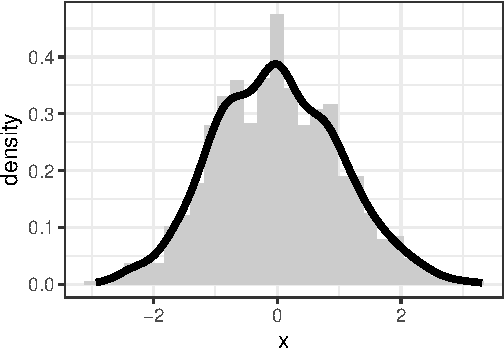
\includegraphics{concepts-and-computation_files/figure-latex/unnamed-chunk-1-1.pdf}

While this variable has a particular location (about zero), we can imagine shifting it left or right. The figure below shows some possible shifts. We could shift it way to the left, so that it's ``about -6'' or a little bit to the right so that it's ``about two.''

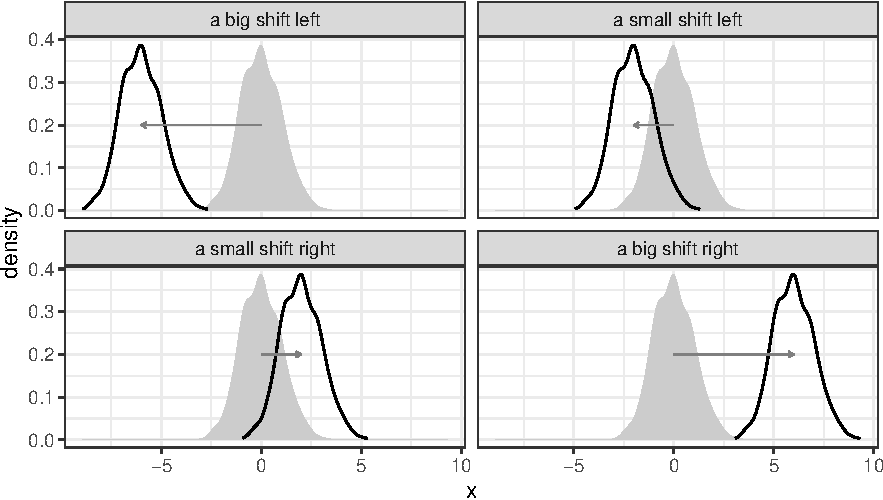
\includegraphics{concepts-and-computation_files/figure-latex/unnamed-chunk-2-1.pdf}

We can also imagine increasing the scale (more spread) or decreasing the scale (less spread). The figure below shows some possible changes in scale. In each case, the ``give or take'' number is changing.

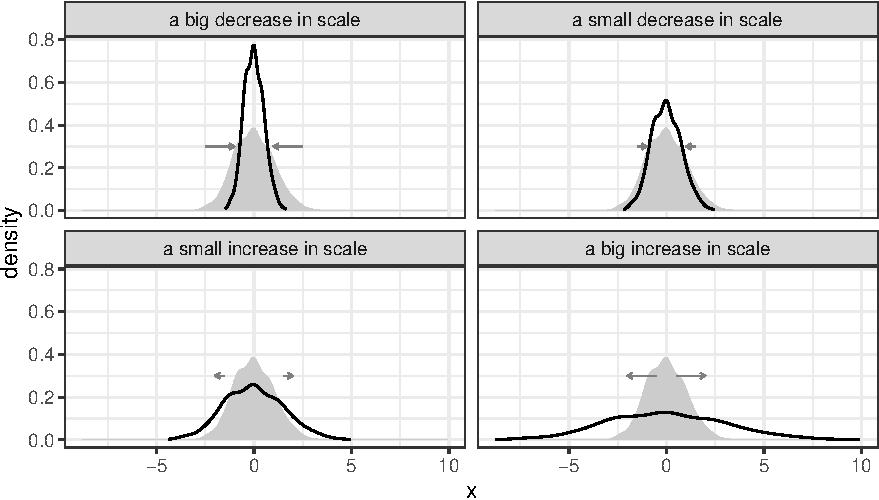
\includegraphics{concepts-and-computation_files/figure-latex/unnamed-chunk-3-1.pdf}

\hypertarget{the-usual-measures}{%
\section{The Usual Measures}\label{the-usual-measures}}

\hypertarget{the-average}{%
\subsection{The Average}\label{the-average}}

The most common measure of the location of a variable is the average.\footnote{Some people refer to the ``average'' as the ``mean''. I prefer to avoid this because the ``mean'' might also refer to the expectation of a random variable. I use ``average'' and ``expected value'' to differentiate these two meanings.} Suppose we have a variable (a list of numbers) \(X = \{x_1, x_2, ..., x_n\}\).

\begin{equation}
\text{average} = \dfrac{\text{the sum of the list}}{\text{the number of entries in the list}} = \dfrac{\sum_{i = 1}^n x_i}{n} \nonumber
\end{equation}

The average is easy to compute and easy to work with mathematically.\footnote{The median, alternatively, is not easy to compute and quite difficult to work with mathematically.}

Unfortunately, the average doesn't have an easy interpretation. The best interpretation, in my mind, is as the balance-point for the data. If we imagine the left-right axis as a teeter-totter and stack the data along the beam according to their values, then the average is the position of the fulcrum that would balance the data-filled beam.

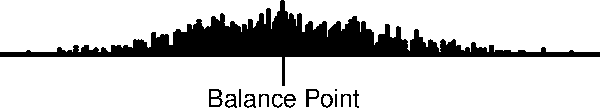
\includegraphics{concepts-and-computation_files/figure-latex/unnamed-chunk-4-1.pdf}

\hypertarget{the-standard-deviation}{%
\subsection{The Standard Deviation}\label{the-standard-deviation}}

The most common measure of scale is the standard deviation (SD). The intuition is subtle, so let's look a a simple example. Rember, our goal is a "give-or-take number.

Suppose we have a list of numbers \(X = \{1, 2, 3, 4, 5\}\). The average of this list is 3, so we can compute the \emph{deviation from average} for each value.

\begin{equation}
\text{deviation from average} = d = \text{value} - \text{average} \nonumber
\end{equation}

In this case, \(d = \{-2, -1, 0, 1, 2\}\).

We want to use these deviations to find a give-or-take number.

Here's an initial idea. Just take the absolute values \(|d| = \{2, 1, 0, 1, 2\}\). These tell us how far each entry falls away from the average. Then we could average the absolute devations to find how far a typical entries falls away from the average of the list. In this case, we get 1.2. This is reasonable approach and we'll refer to it as the average absolute devation or a.a.d. (It turns out that the a.a.d. isn't a common quantity, so I don't elevate it with an all-caps acronym.)

The a.a.d. has one big problem--it uses an absolute value. This introduces some computational and mathematical difficulties.\footnote{Here's the gist: If you take an entry and slide it up and down (i.e., make it larger or smaller), then the a.a.d. moves up and down as well. This is fine, except the a.a.s. doesn't respond smoothly. The figure to the right shows what happens as we move the first entry on the list above around--notice the kink! The derivative of the a.a.d. isn't define here (i.e., there are lots of tangents). This makes things hard mathematically.}

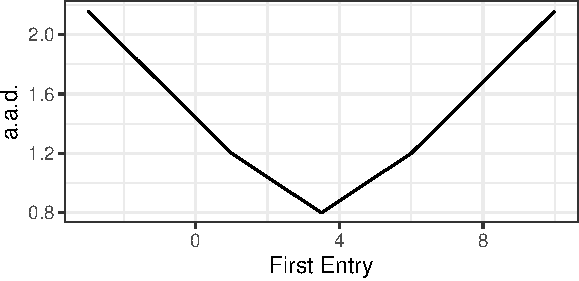
\includegraphics{concepts-and-computation_files/figure-latex/unnamed-chunk-5-1.pdf}

So let's do something similar. Rather than take the absolute value, let's square the deviations, take the average, and then undo the square at the end, so that \(\text{SD} = \sqrt{\text{avg}(d^2)}\).

Sometimes taking the (3) square root of (2) the average of (1) the squares is called the RMS. In this case, the \textbf{RMS of the deviations from the average is the SD}, so that

\begin{equation}
\text{SD} = \sqrt{\text{avg}(d^2)} = \sqrt{\dfrac{(x_i - \text{avg}(X))^2}{n}} = \text{RMS of deviations from average}. \nonumber
\end{equation}

\noindent The SD moves smoothly as you move around the entries in the list.

To calculate the SD, first make this little table, with the list of values, the deviations from the average, and the squares of the deviations.

\begin{longtable}[]{@{}rrr@{}}
\toprule
\(X\) & \(d\) & \(d^2\)\tabularnewline
\midrule
\endhead
1 & -2 & 4\tabularnewline
2 & -1 & 1\tabularnewline
3 & 0 & 0\tabularnewline
4 & 1 & 1\tabularnewline
5 & 2 & 4\tabularnewline
\bottomrule
\end{longtable}

Then compute the average of the squares of the deviations, which in this case is 2. Then take the square root of that average, which in this case is about 1.4. Notice that 1.4 is about 1.2 (the a.a.d.). The SD is bounded (weakly) below by the a.a.s., but they'll usually be close, so we can think of the SD as how far a typical point falls away from the average.

\hypertarget{robust-alternatives}{%
\section{Robust Alternatives}\label{robust-alternatives}}

The average and the SD are mathematically nice. But they are not robust. Seemingly innocuous changes in the variable can lead to large changes in the average and SD.\footnote{The mathmatical ease and the substantive fragility are related.}

We can definite robustness more concretely: How many observations do I need to corrupt to make the summary arbitrarily large?

Suppose the toy variable \(X = \{0.1, -0.6, 1.1, 1.3, 0.2\}\). If I replace the first entry (0.1) with 1, 5, 10, 50, and so on, what happens to the average and SD? The table below shows that we can easily manipulate the average and SD by changing only one data point. In this sense, the average and SD are \textbf{fragile}.

\begin{longtable}[]{@{}lrr@{}}
\toprule
Summary & Average & SD\tabularnewline
\midrule
\endhead
Actual Data Set & 0.42 & 0.70\tabularnewline
First entry of \(X\) replaced with 1 & 0.60 & 0.71\tabularnewline
\ldots{}with 5 & 1.40 & 1.92\tabularnewline
\ldots{}with 10 & 2.40 & 3.86\tabularnewline
\ldots{}with 50 & 10.40 & 19.81\tabularnewline
\ldots{}with 100 & 20.40 & 39.81\tabularnewline
\ldots{}with 500 & 100.40 & 199.80\tabularnewline
\ldots{}with 1,000 & 200.40 & 399.80\tabularnewline
\bottomrule
\end{longtable}

If corrupted data present a problem, then what do we mean by ``corrupt''? There are (at least) three ways to imagine corrupting a measurement.

\begin{enumerate}
\def\labelenumi{\arabic{enumi}.}
\tightlist
\item
  First, perhaps we have a data entry error. While entering data in a spreadsheet, you entered the number 50,000 into the ``hours spent watching the news per day'' variable instead of the ``income'' variable.
\item
  Second, perhaps our measurement procedure is noisy. Suppose we are coding Twitter posts by their support or opposition to President Trump. Our algorithm might interpret a sarcastic take as support when it actually presented intense opposition.
\item
  Third, the substantive model might not apply to a particular observation. Take Clark and Golder's project as an eplxame. They suggest that SMD systems should only have two parties. Indeed, this is a strong theoretical equilibirum. However, it might take several elections to reach this equilibrium. Parties might take several years to coordinate and consolodate. If we include a new democracy in the data set, then we might consider these data ``corrupted'' since the conceptual model doesn't apply (yet).
\end{enumerate}

The average and SD respond to even a small amount of corrupt data.

As an alternative to the average, we might use the median, which is more robust. The median is the/a number which splits the values in half, so that equal numbers of entries lie above and below the median.

We have two common robust alternatives to the SD. The interquartile range (IQR) is the difference between the 25th and 75th quantiles. The median absolute deviation (MAD) is the median of the absolute values of the deviations from the \textbf{median} (almost the a.a.d., but using the medians in place of averages). It turns out that multiplying the MAD by 1.4826 makes it similar to the SD in many dataset, so it's common to rescale it.

To illustrate the robustness of each of our measures of location and scale, let's imagine a variable with 10 observations \(X = \{-1.1, 1.5, -1, -0.1, -1.1, 0, -0.4, 0, 0.8, 0.4\}\). Let's see how the measures change as we corrupt more and more of the observations.

\begin{longtable}[]{@{}llrrrrr@{}}
\toprule
Summary & \% Corrupted & Average & SD & Median & IQR & MAD\tabularnewline
\midrule
\endhead
Actual Data Set & 0\% & -0.10 & 0.81 & -0.05 & 1.15 & 0.96\tabularnewline
First entry of \(X\) replaced with 100 & 10\% & 10.01 & 30.01 & 0.00 & 1.03 & 0.89\tabularnewline
First two entries\ldots{} & 20\% & 19.86 & 40.07 & 0.00 & 1.03 & 0.89\tabularnewline
First three entries\ldots{} & 30\% & 29.96 & 45.85 & 0.20 & 75.28 & 0.89\tabularnewline
First four entries\ldots{} & 40\% & 39.97 & 49.02 & 0.60 & 100.00 & 2.00\tabularnewline
First five entries\ldots{} & 50\% & 50.08 & 49.92 & 50.40 & 99.90 & 73.54\tabularnewline
First six entries\ldots{} & 60\% & 60.08 & 48.89 & 100.00 & 99.50 & 0.00\tabularnewline
\bottomrule
\end{longtable}

This table illustrates that while the average and SD respond to \emph{any} corruption, the median, IQR, and MAD remain reasonable summaries of the uncorrupted variable with 40\%, 20\%, and 30\% of the data corrupted, respectively. T

The percent of the data that one can corrupt before they can make the measure arbitrarily large is called the \textbf{breakdown point}. Here are the breakdown points for our measures:

\begin{longtable}[]{@{}ll@{}}
\toprule
Measure & Breakdown Point\tabularnewline
\midrule
\endhead
Average & 0\%\tabularnewline
SD & 0\%\tabularnewline
Median & 50\%\tabularnewline
IQR & 25\%\tabularnewline
MAD & 50\%\tabularnewline
\bottomrule
\end{longtable}

As you can see, the median and the MAD are highly robust--they achieve the theoretical maximum breakdown point.

\hypertarget{computation-in-r}{%
\section{Computation in R}\label{computation-in-r}}

We can easily calculate all these measures of location and scale in R.\footnote{For reasons I don't want to deal with now, R uses the formula \(SD = \sqrt{\dfrac{(x_i - \text{avg}(X))^2}{n - 1}}\) rather than \(\sqrt{\dfrac{(x_i - \text{avg}(X))^2}{n}}\). This means that R's SD will be slightly larger than the SD with my formula. This difference will be tiny in data sets with a typical number of observations.}

\begin{Shaded}
\begin{Highlighting}[]
\CommentTok{# create variable x = \{1, 2, 3, 4, 5\}}
\NormalTok{x <-}\StringTok{ }\DecValTok{1}\OperatorTok{:}\DecValTok{5}

\CommentTok{# compute measures of location and scale}
\KeywordTok{mean}\NormalTok{(x)  }\CommentTok{# average}
\end{Highlighting}
\end{Shaded}

\begin{verbatim}
## [1] 3
\end{verbatim}

\begin{Shaded}
\begin{Highlighting}[]
\KeywordTok{sd}\NormalTok{(x) }\CommentTok{# SD; see sidenote}
\end{Highlighting}
\end{Shaded}

\begin{verbatim}
## [1] 1.581139
\end{verbatim}

\begin{Shaded}
\begin{Highlighting}[]
\KeywordTok{median}\NormalTok{(x)  }\CommentTok{# median}
\end{Highlighting}
\end{Shaded}

\begin{verbatim}
## [1] 3
\end{verbatim}

\begin{Shaded}
\begin{Highlighting}[]
\KeywordTok{IQR}\NormalTok{(x)  }\CommentTok{# IQR}
\end{Highlighting}
\end{Shaded}

\begin{verbatim}
## [1] 2
\end{verbatim}

\begin{Shaded}
\begin{Highlighting}[]
\KeywordTok{mad}\NormalTok{(x)  }\CommentTok{# MAD, rescaled by 1.4826}
\end{Highlighting}
\end{Shaded}

\begin{verbatim}
## [1] 1.4826
\end{verbatim}

\begin{Shaded}
\begin{Highlighting}[]
\KeywordTok{mad}\NormalTok{(x, }\DataTypeTok{constant =} \DecValTok{1}\NormalTok{)  }\CommentTok{# MAD, not rescaled}
\end{Highlighting}
\end{Shaded}

\begin{verbatim}
## [1] 1
\end{verbatim}

The functions above work nicely for computing on whole variables. But in most cases, we are interested in comparing the summaries across groups.

Take the nominate data set for example.

\begin{Shaded}
\begin{Highlighting}[]
\CommentTok{# load packages}
\KeywordTok{library}\NormalTok{(tidyverse)}

\CommentTok{# load nominate data}
\NormalTok{df <-}\StringTok{ }\KeywordTok{read_rds}\NormalTok{(}\StringTok{"data/nominate.rds"}\NormalTok{) }\OperatorTok
\StringTok{  }\KeywordTok{glimpse}\NormalTok{()}
\end{Highlighting}
\end{Shaded}

\begin{verbatim}
## Observations: 7,080
## Variables: 7
## $ congress <int> 100, 100, 100, 100, 100, 100, 100, 100, 100, 100, 100...
## $ chamber  <chr> "House", "House", "House", "House", "House", "House",...
## $ state    <chr> "AL", "AL", "AL", "AL", "AL", "AL", "AL", "AK", "AZ",...
## $ district <int> 2, 4, 3, 5, 6, 1, 7, 1, 2, 3, 5, 4, 1, 3, 1, 4, 2, 36...
## $ party    <fct> Republican, Democrat, Democrat, Democrat, Democrat, R...
## $ name     <chr> "DICKINSON, William Louis", "BEVILL, Tom", "NICHOLS, ...
## $ ideology <dbl> 0.398, -0.213, -0.042, -0.175, -0.060, 0.373, -0.085,...
\end{verbatim}

For these data, we might want to know the average ideology for Republicans and Democrats. We could do it the hard way.

\begin{Shaded}
\begin{Highlighting}[]
\CommentTok{# create a data frame with only republicans}
\NormalTok{rep_df <-}\StringTok{ }\NormalTok{df }\OperatorTok
\StringTok{  }\KeywordTok{filter}\NormalTok{(party }\OperatorTok{==}\StringTok{ "Republican"}\NormalTok{) }

\CommentTok{# compute average}
\KeywordTok{mean}\NormalTok{(rep_df}\OperatorTok{$}\NormalTok{ideology, }\DataTypeTok{na.rm =} \OtherTok{TRUE}\NormalTok{)}
\end{Highlighting}
\end{Shaded}

\begin{verbatim}
## [1] 0.4213385
\end{verbatim}

But this is tedious, especially if we wanted to do it by party and Congress.

To compute these summaries for lots of subsets of the data, we have the \texttt{group\_by()/summarize()} workflow.

\texttt{group\_by()} defines several groups in the data frame. The first argument is the data frame to group (but we'll \texttt{\%\textgreater{}\%} it in). The remaining arguments are the grouping variables. You can think if the groups as a footnote at the bottom of the data set that just mentions the variables that define the groups of interest. Whenever we act (in the wrangling sense) on the data set and the action makes sense in the context of groups, the action will happen by group.

After grouping, we use \texttt{summarize()} to create summaries for each group. The first argument is the data frame to summarize (but we'll \texttt{\%\textgreater{}\%} it in). The remaining arguments are the summarizes to compute. The names of the remaining arguments become variables in the resulting data frame.

\begin{Shaded}
\begin{Highlighting}[]
\NormalTok{smry_df <-}\StringTok{ }\NormalTok{df }\OperatorTok
\StringTok{  }\CommentTok{# group by party and congress}
\StringTok{  }\KeywordTok{group_by}\NormalTok{(party, congress) }\OperatorTok
\StringTok{  }\CommentTok{# compute all of our measures of location and scale}
\StringTok{  }\KeywordTok{summarize}\NormalTok{(}\DataTypeTok{average =} \KeywordTok{mean}\NormalTok{(ideology, }\DataTypeTok{na.rm =} \OtherTok{TRUE}\NormalTok{),}
            \DataTypeTok{sd =} \KeywordTok{sd}\NormalTok{(ideology, }\DataTypeTok{na.rm =} \OtherTok{TRUE}\NormalTok{), }
            \DataTypeTok{median =} \KeywordTok{median}\NormalTok{(ideology, }\DataTypeTok{na.rm =} \OtherTok{TRUE}\NormalTok{), }
            \DataTypeTok{iqr =} \KeywordTok{IQR}\NormalTok{(ideology, }\DataTypeTok{na.rm =} \OtherTok{TRUE}\NormalTok{),}
            \DataTypeTok{mad =} \KeywordTok{mad}\NormalTok{(ideology, }\DataTypeTok{na.rm =} \OtherTok{TRUE}\NormalTok{),}
            \DataTypeTok{mad1 =} \KeywordTok{mad}\NormalTok{(ideology, }\DataTypeTok{constant =} \DecValTok{1}\NormalTok{, }\DataTypeTok{na.rm =} \OtherTok{TRUE}\NormalTok{)) }\OperatorTok
\StringTok{  }\CommentTok{# quick look at our work}
\StringTok{  }\KeywordTok{glimpse}\NormalTok{()}
\end{Highlighting}
\end{Shaded}

\begin{verbatim}
## Observations: 32
## Variables: 8
## Groups: party [2]
## $ party    <fct> Democrat, Democrat, Democrat, Democrat, Democrat, Dem...
## $ congress <int> 100, 101, 102, 103, 104, 105, 106, 107, 108, 109, 110...
## $ average  <dbl> -0.3092901, -0.3130075, -0.3142407, -0.3333065, -0.36...
## $ sd       <dbl> 0.1653092, 0.1664293, 0.1658089, 0.1609726, 0.1524251...
## $ median   <dbl> -0.3200, -0.3200, -0.3200, -0.3360, -0.3815, -0.3835,...
## $ iqr      <dbl> 0.22750, 0.22600, 0.23025, 0.24000, 0.20550, 0.17850,...
## $ mad      <dbl> 0.1675338, 0.1719816, 0.1690164, 0.1793946, 0.1490013...
## $ mad1     <dbl> 0.1130, 0.1160, 0.1140, 0.1210, 0.1005, 0.0895, 0.087...
\end{verbatim}

We can plot this measures to get a sense of how they change over time. Notice that \texttt{mad} (rescaled by multiplying by 1.4826) closely corresponds to the SD, but \texttt{mad1} (not rescaled) is much smaller.

\begin{Shaded}
\begin{Highlighting}[]
\CommentTok{# wrangle the data for plotting}
\NormalTok{gg_df <-}\StringTok{ }\NormalTok{smry_df }\OperatorTok
\StringTok{  }\KeywordTok{pivot_longer}\NormalTok{(average}\OperatorTok{:}\NormalTok{mad1, }\DataTypeTok{names_to =} \StringTok{"measure"}\NormalTok{) }\OperatorTok
\StringTok{  }\KeywordTok{mutate}\NormalTok{(}\DataTypeTok{measure_of =} \KeywordTok{ifelse}\NormalTok{(measure }\OperatorTok\StringTok{ }\KeywordTok{c}\NormalTok{(}\StringTok{"average"}\NormalTok{, }\StringTok{"median"}\NormalTok{), }\StringTok{"location"}\NormalTok{, }\StringTok{"scale"}\NormalTok{)) }\OperatorTok
\StringTok{  }\KeywordTok{glimpse}\NormalTok{()}
\end{Highlighting}
\end{Shaded}

\begin{verbatim}
## Observations: 192
## Variables: 5
## Groups: party [2]
## $ party      <fct> Democrat, Democrat, Democrat, Democrat, Democrat, D...
## $ congress   <int> 100, 100, 100, 100, 100, 100, 101, 101, 101, 101, 1...
## $ measure    <chr> "average", "sd", "median", "iqr", "mad", "mad1", "a...
## $ value      <dbl> -0.3092901, 0.1653092, -0.3200000, 0.2275000, 0.167...
## $ measure_of <chr> "location", "scale", "location", "scale", "scale", ...
\end{verbatim}

\begin{Shaded}
\begin{Highlighting}[]
\CommentTok{# plot the measures of location and scale}
\KeywordTok{ggplot}\NormalTok{(gg_df, }\KeywordTok{aes}\NormalTok{(}\DataTypeTok{x =}\NormalTok{ congress, }\DataTypeTok{y =}\NormalTok{ value, }\DataTypeTok{color =}\NormalTok{ measure)) }\OperatorTok{+}\StringTok{ }
\StringTok{  }\KeywordTok{geom_line}\NormalTok{() }\OperatorTok{+}\StringTok{ }
\StringTok{  }\KeywordTok{facet_grid}\NormalTok{(}\DataTypeTok{cols =} \KeywordTok{vars}\NormalTok{(party), }\DataTypeTok{rows =} \KeywordTok{vars}\NormalTok{(measure_of), }\DataTypeTok{scales =} \StringTok{"free_y"}\NormalTok{)}
\end{Highlighting}
\end{Shaded}

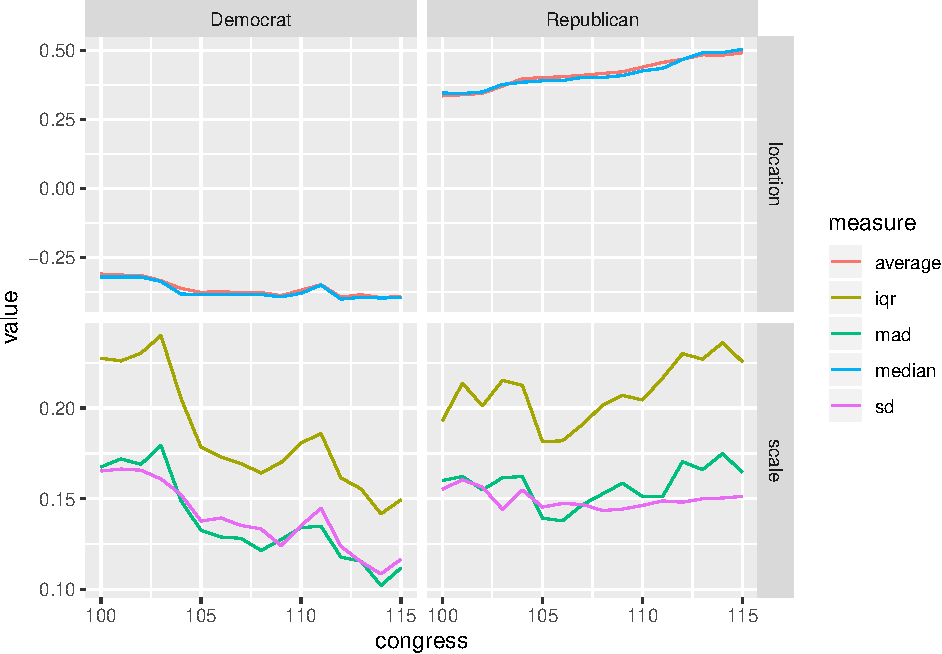
\includegraphics{concepts-and-computation_files/figure-latex/unnamed-chunk-13-1.pdf}

\hypertarget{the-normal-model}{%
\chapter{The Normal Model}\label{the-normal-model}}

\hypertarget{the-intuition-1}{%
\section{The Intuition}\label{the-intuition-1}}

Last week, we used the average and SD to reduce and entire variable to two summaries. We use the average and SD to fill in the following sentence: ``The values are about \_\_\_\_\_\_\_\_, give or take \_\_\_\_\_\_\_\_ or so.''

This week, we add an additional assumption. This week, we also say that the histogram of the variable follows the normal curve. The normal curve is a bell-shaped curve with a particular equation. There are two varieties. There is a general, parameterized normal distibution that can move left and right (i.e., change location) and grow wider or taller (i.e., change scale)

\hypertarget{the-normal-curves}{%
\section{The Normal Curve(s)}\label{the-normal-curves}}

There are two particular normal curves that we care about

\begin{enumerate}
\def\labelenumi{\arabic{enumi}.}
\tightlist
\item
  \textbf{the normal curve}, which has a location and scale parameter that we can specify: \(f(x | \mu, \sigma) = \phi(x | \mu, \sigma) = \frac{1}{{\sigma \sqrt {2\pi } }}e^\frac{{ - \left( {x - \mu } \right)^2 }}{2\sigma ^2 }\)
\item
  \textbf{the \emph{standard} normal curve}, with the location and scale parameters fixed: \(f(x | \mu = 0, \sigma = 1) = \phi(x | \mu = 0, \sigma = 1) = \frac{1}{{\sqrt {2\pi } }}e^\frac{{ - x ^2 }}{2}\)
\end{enumerate}

These equations are complicated. Instead of memorizing them or working carefully through the math, just understand (for now) that the normal curve has an equation that exactly characterizes it. The figure below shows the \emph{standard} normal curve (\(\mu = 0\) and \(\sigma = 1\)) and several other paramaterizations.

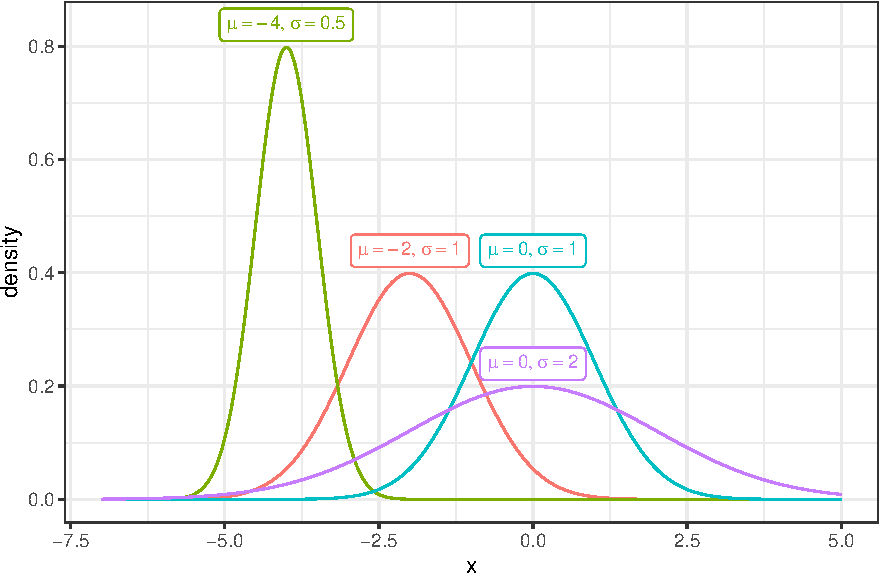
\includegraphics{concepts-and-computation_files/figure-latex/unnamed-chunk-15-1.pdf}

\hypertarget{the-empirical-rule}{%
\section{The Empirical Rule}\label{the-empirical-rule}}

It turns out that many variable's have a histogram that resembles the normal curve. Because of this, the normal curve can sometimes serve as an effective model for these variables.

For example, NOMINATE ideology scores for Republicans in the 115th Congress roughly follow the normal curve.

\begin{Shaded}
\begin{Highlighting}[]
\NormalTok{df <-}\StringTok{ }\KeywordTok{read_rds}\NormalTok{(}\StringTok{"data/nominate.rds"}\NormalTok{) }\OperatorTok
\StringTok{  }\KeywordTok{filter}\NormalTok{(party }\OperatorTok{==}\StringTok{ "Democrat"}\NormalTok{, congress }\OperatorTok{==}\StringTok{ }\DecValTok{115}\NormalTok{) }

\KeywordTok{ggplot}\NormalTok{(df, }\KeywordTok{aes}\NormalTok{(}\DataTypeTok{x =}\NormalTok{ ideology)) }\OperatorTok{+}\StringTok{ }
\StringTok{  }\KeywordTok{geom_histogram}\NormalTok{() }
\end{Highlighting}
\end{Shaded}

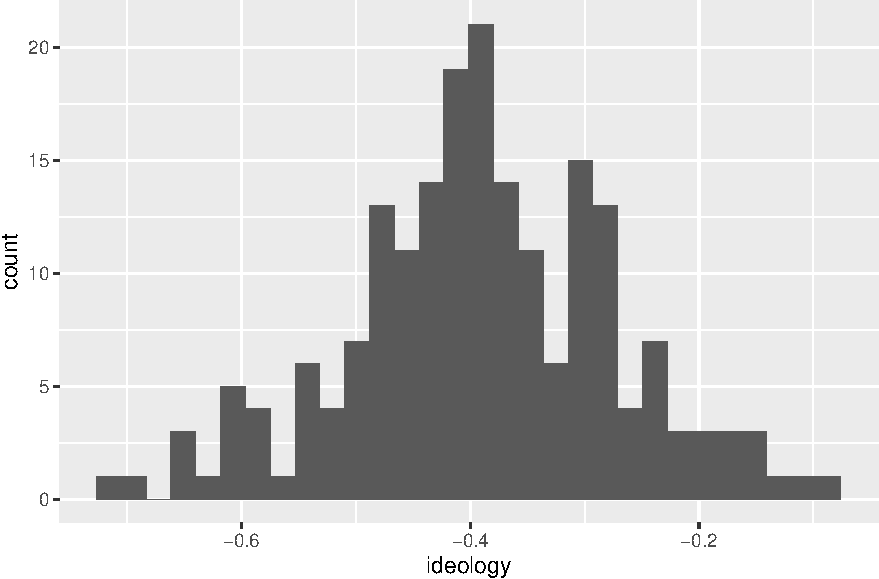
\includegraphics{concepts-and-computation_files/figure-latex/unnamed-chunk-16-1.pdf}

However, the ideology scores for both Republicans and Democrats together does not follow a normal curve.

\begin{Shaded}
\begin{Highlighting}[]
\NormalTok{df <-}\StringTok{ }\KeywordTok{read_rds}\NormalTok{(}\StringTok{"data/nominate.rds"}\NormalTok{)}

\KeywordTok{ggplot}\NormalTok{(df, }\KeywordTok{aes}\NormalTok{(}\DataTypeTok{x =}\NormalTok{ ideology)) }\OperatorTok{+}\StringTok{ }
\StringTok{  }\KeywordTok{geom_histogram}\NormalTok{() }
\end{Highlighting}
\end{Shaded}

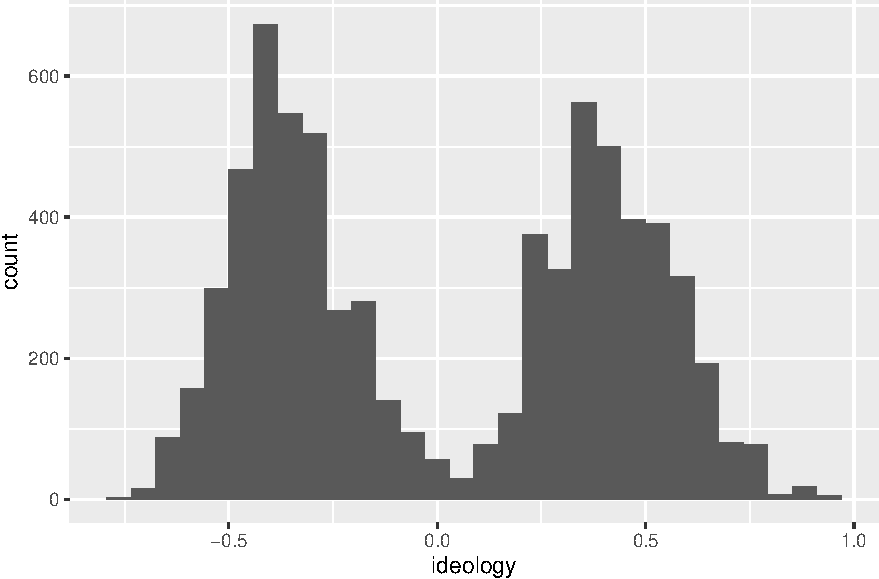
\includegraphics{concepts-and-computation_files/figure-latex/unnamed-chunk-17-1.pdf}

The histograms of ENEP by electoral system and social heterogeneity deviate slightly from the normal curve.

\begin{verbatim}
## Observations: 1,161
## Variables: 4
## $ x                    <dbl> 1.23, 1.33, 1.43, 1.53, 1.63, 1.73, 1.83,...
## $ density              <dbl> 0.02616495, 0.02960818, 0.03338541, 0.037...
## $ electoral_system     <fct> Large-Magnitude PR, Large-Magnitude PR, L...
## $ social_heterogeneity <fct> Bottom 3rd of ENEG, Bottom 3rd of ENEG, B...
\end{verbatim}

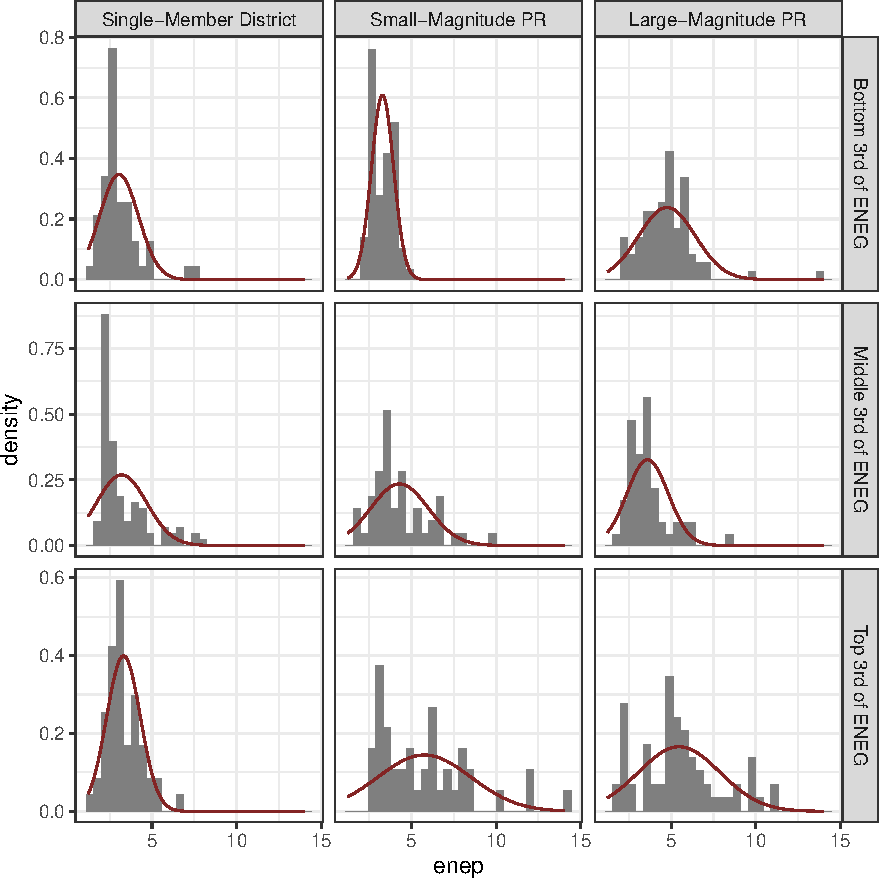
\includegraphics{concepts-and-computation_files/figure-latex/unnamed-chunk-18-1.pdf}

If the variable seems to follow the normal curve, then we have the following rules:

\begin{itemize}
\tightlist
\item
  About \emph{68\%} of the data (i.e., ``most'') fall within \textbf{1 SD} of the average.
\item
  About \emph{95\%} of the data (i.e., ``almost all'') fall within \textbf{2 SDs} of the average.
\end{itemize}

We can evaluate this rule with the parties data above. Some of the nine hisgrams follow the normal curve quite well (e.g., lower-left). Other's seem to meaningfully deviate from the normal curve (e.g., middle-left).

The table below shows the actual percent of the variable that falls within one and two SDs of the average for each histogram. As you can see, for the lower-left panel (SMD, Top 3rd), the empircal rule of 68\% and 95\% matches the actual values of 74\% and 98\% fairly well. For the middle-left panel (SMD, Middle 3rd), the empirical rule matches the actual values of 87\% and 93\% less well.

Across all histograms, it seems fair that the empirical rule works as a rough approximation, even for histograms that meaningfully deviate from the normal curve.

\begin{longtable}[]{@{}llll@{}}
\toprule
Electoral System & Social Heterogeneity & within 1 SD & within 2 SDs\tabularnewline
\midrule
\endhead
Single-Member District & Bottom 3rd of ENEG & 87\% & 96\%\tabularnewline
Single-Member District & Middle 3rd of ENEG & 87\% & 93\%\tabularnewline
Single-Member District & Top 3rd of ENEG & 74\% & 98\%\tabularnewline
Small-Magnitude PR & Bottom 3rd of ENEG & 68\% & 97\%\tabularnewline
Small-Magnitude PR & Middle 3rd of ENEG & 73\% & 96\%\tabularnewline
Small-Magnitude PR & Top 3rd of ENEG & 76\% & 93\%\tabularnewline
Large-Magnitude PR & Bottom 3rd of ENEG & 80\% & 98\%\tabularnewline
Large-Magnitude PR & Middle 3rd of ENEG & 77\% & 96\%\tabularnewline
Large-Magnitude PR & Top 3rd of ENEG & 65\% & 97\%\tabularnewline
\bottomrule
\end{longtable}

\hypertarget{the-normal-approximation}{%
\section{The Normal Approximation}\label{the-normal-approximation}}

If our normal model summarizes a histogram well, then we can use the model to estimate the percent of the observations that fall in a given range. There are two approaches:

Just like we add up the area of the bars to compute percentages with a histogram, \textbf{we add up the area under the normal curve to approximate percentages.}

\begin{enumerate}
\def\labelenumi{\arabic{enumi}.}
\tightlist
\item
  Use a normal table from a textbook. Because the table is for the standard normal curve, we need to \textbf{re-locate and re-scale the data to fit the standard normal curve}.
\item
  Use the \texttt{pnorm()} function in R. Because this function is parameterized with location and scale, we can simple \textbf{re-locate and re-scale the curve to fit the data}.
\end{enumerate}

\hypertarget{normal-table}{%
\subsection{Normal Table}\label{normal-table}}

Normal tables offer an antiquated method to use the normal distribution to approximate percentages. Because we cannot have a normal table for all possible locations and scales, we have one: the standard normal table, which works for a variable with an average of zero and an SD of one.

This seems limiting, but it turns out that we can easily re-locate and re-scale any value to match the standard normal curve. We simply subtract the average and divide by the SD. We call this new value a \emph{z}-score.

\(z\text{-score} = \dfrac{\text{value} - \text{average}}{\text{SD}}\)

FSuppose we have the list \(X = \{1, 2, 3, 4, 5\}\). Then the average is 3, and the SD is about 1.26. We can compute the \emph{z}score for the first entry 1 as \(\frac{1 - 3}{1.25} \approx -1.58\). Similarly, we can convert the entire list to \emph{z}-scores and get \(Z = \{1.59, -0.79, 0.00, 0.79, 1.59\}\). If you compute the average and SD of the list \(Z\), you will find zero and one, respectively.

We can then use a normal table to compute areas under the normal curve between (or above or below) these values of \(z\). There are two types of normal tables.

\begin{enumerate}
\def\labelenumi{\arabic{enumi}.}
\tightlist
\item
  Some tables report the percent (or proportion) of the normal curve \textbf{below} a particular value \(z\).
\item
  Other tables report the percent (or proportion) of the normal curve \textbf{between} a particular value \(z\) and \(-z\). (The normal table on p.~A-104 of FPP works this way.)
\end{enumerate}

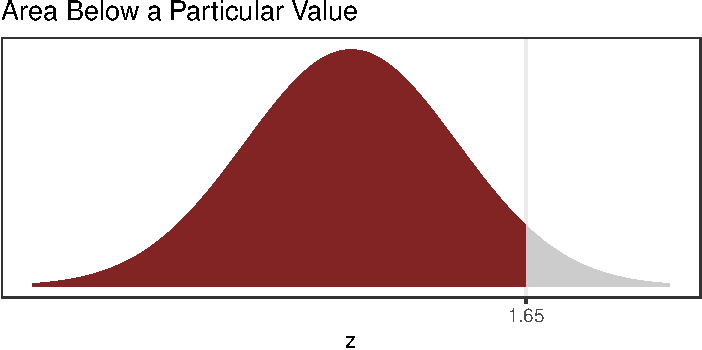
\includegraphics{concepts-and-computation_files/figure-latex/unnamed-chunk-20-1.pdf}

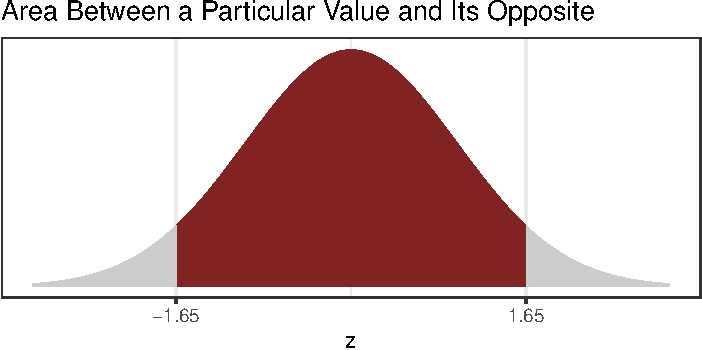
\includegraphics{concepts-and-computation_files/figure-latex/unnamed-chunk-21-1.pdf}

Either table works, but you must know what type of table you are working with. Depending on the question, one type might offer a more direct solution.

Here's a small normal table for a few values of \(z\) that uses both approaches.

\begin{longtable}[]{@{}rlll@{}}
\toprule
\emph{z} & \% less than \emph{z} & \% between \emph{-z} and \emph{z} & Status\tabularnewline
\midrule
\endhead
0.00 & 50\% & 0\% &\tabularnewline
0.10 & 54\% & 8\% &\tabularnewline
0.20 & 58\% & 16\% &\tabularnewline
0.30 & 62\% & 24\% &\tabularnewline
0.40 & 66\% & 31\% &\tabularnewline
0.50 & 69\% & 38\% &\tabularnewline
0.75 & 77\% & 55\% &\tabularnewline
1.00 & 84\% & 68\% & Important\tabularnewline
1.50 & 93\% & 87\% &\tabularnewline
1.64 & 95\% & 90\% & Important\tabularnewline
1.96 & 98\% & 95\% & Important\tabularnewline
2.00 & 98\% & 95\% & Important\tabularnewline
3.00 & 100\% & 100\% &\tabularnewline
\bottomrule
\end{longtable}

In order to use the table to find the area between any two values, you need to use the following three rules in combination.

\begin{enumerate}
\def\labelenumi{\arabic{enumi}.}
\tightlist
\item
  The normal table gives the area (i) below \(z\) or (ii) between \(-z\) and \(z\).
\item
  The area under the entire normal curve is 1 or 100\%.
\item
  The normal curve is symetric, so that the area to the right of \(z\) equals the area to the left of \(-z\).
\end{enumerate}

\hypertarget{pnorm}{%
\subsection{\texorpdfstring{\texttt{pnorm()}}{pnorm()}}\label{pnorm}}

The \texttt{pnorm()} function in R return the area under the normal curve less than \(z\). By default, it uses the standard normal curve, but you can specify a \texttt{mean} and \texttt{sd} if you prefer to re-locate and/or re-scale the curve to fit your values.

\begin{Shaded}
\begin{Highlighting}[]
\CommentTok{# area under the std. normal curve less than 1}
\KeywordTok{pnorm}\NormalTok{(}\DecValTok{1}\NormalTok{)}
\end{Highlighting}
\end{Shaded}

\begin{verbatim}
## [1] 0.8413447
\end{verbatim}

\begin{Shaded}
\begin{Highlighting}[]
\CommentTok{# area under the a normal curve (with average of 1 and SD of 4) less than 1}
\KeywordTok{pnorm}\NormalTok{(}\DecValTok{1}\NormalTok{, }\DataTypeTok{mean =} \DecValTok{1}\NormalTok{, }\DataTypeTok{sd =} \DecValTok{4}\NormalTok{)}
\end{Highlighting}
\end{Shaded}

\begin{verbatim}
## [1] 0.5
\end{verbatim}

\begin{Shaded}
\begin{Highlighting}[]
\CommentTok{# area between -1.64 and 1.64}
\KeywordTok{pnorm}\NormalTok{(}\FloatTok{1.64}\NormalTok{) }\OperatorTok{-}\StringTok{ }\KeywordTok{pnorm}\NormalTok{(}\OperatorTok{-}\FloatTok{1.64}\NormalTok{)}
\end{Highlighting}
\end{Shaded}

\begin{verbatim}
## [1] 0.8989948
\end{verbatim}

\hypertarget{exactly-percentages}{%
\subsection{Exactly Percentages}\label{exactly-percentages}}

To actually compute percentages, we can create a function that works just like \texttt{pnorm()}, but it returns the percent \emph{of the data} that fall below a particular value. The most convenient method is to create an "empirical cumulative distribution function*.

This function is somewhat confusing. The \texttt{ecdf()} function does not return the proportion below its argument. Instead, it creates a function that returns the percent below its argument. If we have a numeric vector \texttt{x}, then \texttt{ecdf(x)} is a function! Let that settle in\ldots{} both \texttt{ecdf} and \texttt{ecdf(x)} are function. The function \texttt{ecdf} (I'm dropping the \texttt{()} for clarity) is a function \emph{that creates a function}, and \texttt{ecdf(x)()} (I'm including the \texttt{()}, as usual, for clarity) is a function that returns the percent below.

\begin{Shaded}
\begin{Highlighting}[]
\NormalTok{df <-}\StringTok{ }\KeywordTok{read_rds}\NormalTok{(}\StringTok{"data/nominate.rds"}\NormalTok{) }\OperatorTok
\StringTok{  }\KeywordTok{filter}\NormalTok{(party }\OperatorTok{==}\StringTok{ "Democrat"}\NormalTok{, congress }\OperatorTok{==}\StringTok{ }\DecValTok{115}\NormalTok{) }

\CommentTok{# normal approximation for % of Democrats less than -0.05}
\NormalTok{avg <-}\StringTok{ }\KeywordTok{mean}\NormalTok{(df}\OperatorTok{$}\NormalTok{ideology)}
\NormalTok{sd <-}\StringTok{ }\KeywordTok{sd}\NormalTok{(df}\OperatorTok{$}\NormalTok{ideology)}
\KeywordTok{pnorm}\NormalTok{(}\OperatorTok{-}\FloatTok{0.5}\NormalTok{, }\DataTypeTok{mean =}\NormalTok{ avg, }\DataTypeTok{sd =}\NormalTok{ sd)}
\end{Highlighting}
\end{Shaded}

\begin{verbatim}
## [1] 0.1731597
\end{verbatim}

\begin{Shaded}
\begin{Highlighting}[]
\CommentTok{# exact % of Democrats less than -0.05}
\KeywordTok{ecdf}\NormalTok{(df}\OperatorTok{$}\NormalTok{ideology)(}\OperatorTok{-}\FloatTok{0.5}\NormalTok{)}
\end{Highlighting}
\end{Shaded}

\begin{verbatim}
## [1] 0.1479592
\end{verbatim}

We can also plot the ECDF with ggplot2.

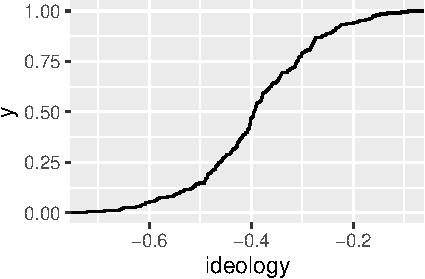
\includegraphics{concepts-and-computation_files/figure-latex/unnamed-chunk-25-1.pdf}

\hypertarget{review-exercises}{%
\section{Review Exercises}\label{review-exercises}}

The plot below show the histograms for the ideology of legislators in the U.S. House by party.

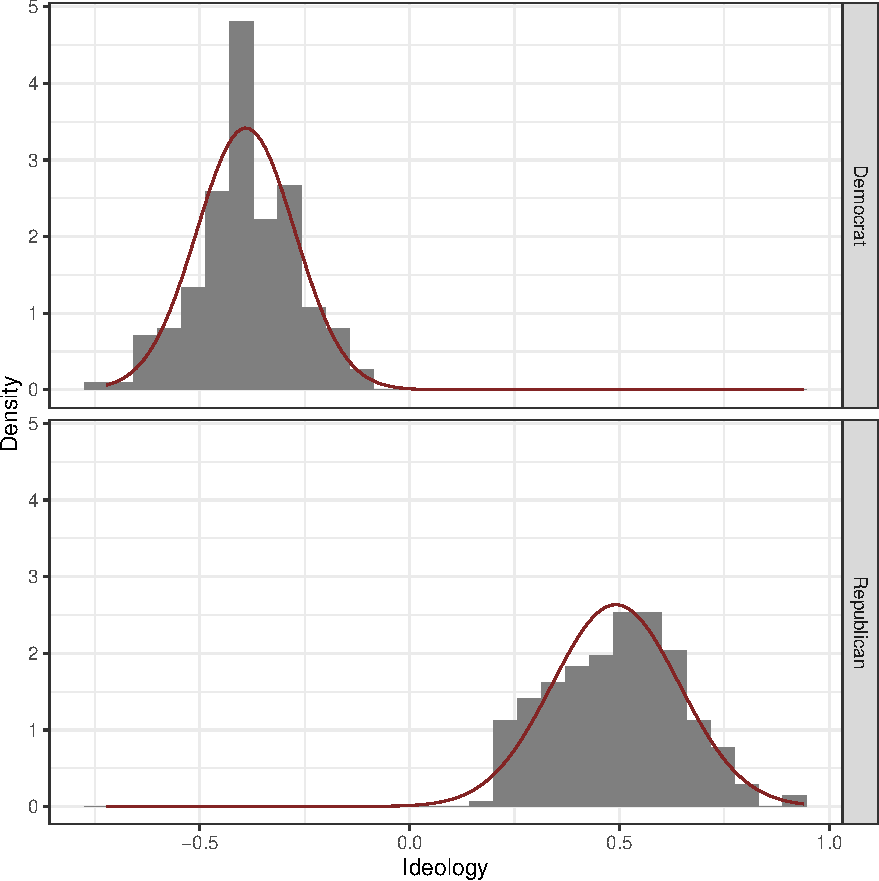
\includegraphics{concepts-and-computation_files/figure-latex/unnamed-chunk-26-1.pdf}

We can compute the average and SD by party.

\begin{longtable}[]{@{}lrr@{}}
\toprule
Party & Average & SD\tabularnewline
\midrule
\endhead
Democrat & -0.39 & 0.12\tabularnewline
Republican & 0.49 & 0.15\tabularnewline
\bottomrule
\end{longtable}

The table below lists some of the leaders of each party and their ideology score. For each leader, use our three approaches to compute the percent of the party that is ``more extreme'' than their leader: inspect the histogram, use the normal approximation, and use R to compute the answer exactly.

\begin{longtable}[]{@{}lllrlll@{}}
\toprule
\begin{minipage}[b]{0.15\columnwidth}\raggedright
Name\strut
\end{minipage} & \begin{minipage}[b]{0.07\columnwidth}\raggedright
Party\strut
\end{minipage} & \begin{minipage}[b]{0.21\columnwidth}\raggedright
Position\strut
\end{minipage} & \begin{minipage}[b]{0.09\columnwidth}\raggedleft
Ideology Score\strut
\end{minipage} & \begin{minipage}[b]{0.11\columnwidth}\raggedright
Inspect Histogram\strut
\end{minipage} & \begin{minipage}[b]{0.13\columnwidth}\raggedright
Normal Approximation\strut
\end{minipage} & \begin{minipage}[b]{0.04\columnwidth}\raggedright
Actual\strut
\end{minipage}\tabularnewline
\midrule
\endhead
\begin{minipage}[t]{0.15\columnwidth}\raggedright
RYAN, Paul D.\strut
\end{minipage} & \begin{minipage}[t]{0.07\columnwidth}\raggedright
Republican\strut
\end{minipage} & \begin{minipage}[t]{0.21\columnwidth}\raggedright
Speaker of the House\strut
\end{minipage} & \begin{minipage}[t]{0.09\columnwidth}\raggedleft
0.56\strut
\end{minipage} & \begin{minipage}[t]{0.11\columnwidth}\raggedright
\strut
\end{minipage} & \begin{minipage}[t]{0.13\columnwidth}\raggedright
\strut
\end{minipage} & \begin{minipage}[t]{0.04\columnwidth}\raggedright
\strut
\end{minipage}\tabularnewline
\begin{minipage}[t]{0.15\columnwidth}\raggedright
MCCARTHY, Kevin\strut
\end{minipage} & \begin{minipage}[t]{0.07\columnwidth}\raggedright
Republican\strut
\end{minipage} & \begin{minipage}[t]{0.21\columnwidth}\raggedright
Majority Leader\strut
\end{minipage} & \begin{minipage}[t]{0.09\columnwidth}\raggedleft
0.46\strut
\end{minipage} & \begin{minipage}[t]{0.11\columnwidth}\raggedright
\strut
\end{minipage} & \begin{minipage}[t]{0.13\columnwidth}\raggedright
\strut
\end{minipage} & \begin{minipage}[t]{0.04\columnwidth}\raggedright
\strut
\end{minipage}\tabularnewline
\begin{minipage}[t]{0.15\columnwidth}\raggedright
SCALISE, Steve\strut
\end{minipage} & \begin{minipage}[t]{0.07\columnwidth}\raggedright
Republican\strut
\end{minipage} & \begin{minipage}[t]{0.21\columnwidth}\raggedright
Majority Whip\strut
\end{minipage} & \begin{minipage}[t]{0.09\columnwidth}\raggedleft
0.56\strut
\end{minipage} & \begin{minipage}[t]{0.11\columnwidth}\raggedright
\strut
\end{minipage} & \begin{minipage}[t]{0.13\columnwidth}\raggedright
\strut
\end{minipage} & \begin{minipage}[t]{0.04\columnwidth}\raggedright
\strut
\end{minipage}\tabularnewline
\begin{minipage}[t]{0.15\columnwidth}\raggedright
McMORRIS RODGERS, Cathy\strut
\end{minipage} & \begin{minipage}[t]{0.07\columnwidth}\raggedright
Republican\strut
\end{minipage} & \begin{minipage}[t]{0.21\columnwidth}\raggedright
Conference Chair\strut
\end{minipage} & \begin{minipage}[t]{0.09\columnwidth}\raggedleft
0.43\strut
\end{minipage} & \begin{minipage}[t]{0.11\columnwidth}\raggedright
\strut
\end{minipage} & \begin{minipage}[t]{0.13\columnwidth}\raggedright
\strut
\end{minipage} & \begin{minipage}[t]{0.04\columnwidth}\raggedright
\strut
\end{minipage}\tabularnewline
\begin{minipage}[t]{0.15\columnwidth}\raggedright
PELOSI, Nancy\strut
\end{minipage} & \begin{minipage}[t]{0.07\columnwidth}\raggedright
Democrat\strut
\end{minipage} & \begin{minipage}[t]{0.21\columnwidth}\raggedright
Minority Leader\strut
\end{minipage} & \begin{minipage}[t]{0.09\columnwidth}\raggedleft
-0.49\strut
\end{minipage} & \begin{minipage}[t]{0.11\columnwidth}\raggedright
\strut
\end{minipage} & \begin{minipage}[t]{0.13\columnwidth}\raggedright
\strut
\end{minipage} & \begin{minipage}[t]{0.04\columnwidth}\raggedright
\strut
\end{minipage}\tabularnewline
\begin{minipage}[t]{0.15\columnwidth}\raggedright
HOYER, Steny Hamilton\strut
\end{minipage} & \begin{minipage}[t]{0.07\columnwidth}\raggedright
Democrat\strut
\end{minipage} & \begin{minipage}[t]{0.21\columnwidth}\raggedright
Minority Whip\strut
\end{minipage} & \begin{minipage}[t]{0.09\columnwidth}\raggedleft
-0.38\strut
\end{minipage} & \begin{minipage}[t]{0.11\columnwidth}\raggedright
\strut
\end{minipage} & \begin{minipage}[t]{0.13\columnwidth}\raggedright
\strut
\end{minipage} & \begin{minipage}[t]{0.04\columnwidth}\raggedright
\strut
\end{minipage}\tabularnewline
\begin{minipage}[t]{0.15\columnwidth}\raggedright
CLYBURN, James Enos\strut
\end{minipage} & \begin{minipage}[t]{0.07\columnwidth}\raggedright
Democrat\strut
\end{minipage} & \begin{minipage}[t]{0.21\columnwidth}\raggedright
Assistant Democratic Leader\strut
\end{minipage} & \begin{minipage}[t]{0.09\columnwidth}\raggedleft
-0.46\strut
\end{minipage} & \begin{minipage}[t]{0.11\columnwidth}\raggedright
\strut
\end{minipage} & \begin{minipage}[t]{0.13\columnwidth}\raggedright
\strut
\end{minipage} & \begin{minipage}[t]{0.04\columnwidth}\raggedright
\strut
\end{minipage}\tabularnewline
\begin{minipage}[t]{0.15\columnwidth}\raggedright
LEWIS, John R.\strut
\end{minipage} & \begin{minipage}[t]{0.07\columnwidth}\raggedright
Democrat\strut
\end{minipage} & \begin{minipage}[t]{0.21\columnwidth}\raggedright
Senior Chief Deputy Minority Whip\strut
\end{minipage} & \begin{minipage}[t]{0.09\columnwidth}\raggedleft
-0.59\strut
\end{minipage} & \begin{minipage}[t]{0.11\columnwidth}\raggedright
\strut
\end{minipage} & \begin{minipage}[t]{0.13\columnwidth}\raggedright
\strut
\end{minipage} & \begin{minipage}[t]{0.04\columnwidth}\raggedright
\strut
\end{minipage}\tabularnewline
\bottomrule
\end{longtable}

\bibliography{book.bib,packages.bib}


\end{document}
